\documentclass[a4paper, french]{article}

%% Language and font encodings
\usepackage{babel}
\usepackage[utf8]{inputenc}
\usepackage[T1]{fontenc}

%% Sets page size and margins
\usepackage[a4paper,top=3cm,bottom=2cm,left=2.5cm,right=2.5cm,marginparwidth=1.75cm]{geometry}
\usepackage{multicol}
\usepackage{parskip}


%% Useful packages
\usepackage{amsmath}
\usepackage{amsfonts}
\usepackage{graphicx}
\graphicspath{ {images/} }
\usepackage[colorinlistoftodos]{todonotes}
\usepackage[colorlinks=true, allcolors=black]{hyperref}
\usepackage{float}
\usepackage{listings}

%% verbatim listings
\usepackage{xparse}
\lstset{basicstyle=\ttfamily}
\NewDocumentCommand{\cword}{v}{%
    \texttt{#1}%
}

\title{ivegotmail -- compte-rendu --\\ Classification Binaire Spam/NoSpam}
\author{Ben Kirane Malik, Mouhoubi Fatima}

\begin{document}
\maketitle
%\begin{multicols}{2}
\setlength{\parskip}{0.1in}
\setlength{\parindent}{15pt}

\begin{abstract}
Nous nous int\'eressons au probl\'eme de classification d'une base de courriers
\'el\'ectroniques (emails).
Nous souhaitons \`a partir du corps d'un email savoir s'il s'agit
d'un spam ou non. Il s'agit d'inf\'erer cette connaissance \`a partir
d'un corpus d'emails avec une approche bas\'ee sur les probabilit\'es
(relation de Bayes). Cette approche est  pr\'esent\'ee en premi\`ere partie.
L'objet de ce compte-rendu est ensuite d'\'etudier diff\'erentes mod\'elisations
avec des descriptions enrichies pour r\'epondre au probl\`eme de classification.
\end{abstract}

\tableofcontents

\section{Classifieur par Inf\'erence Bay\'esienne}
Dans cette partie, pour \'etablir  \`a partir des distributions de
probabilit\'es estim\'ees dans la phase d'apprentissage si un email est
un spam ou non, nous illustrerons une solution \'a cette probl\'ematique
avec un mod\`ele tr\`es simple.
Nous travaillerons tout le long sur deux phases distinctes :
la phase d'apprentissage et la phase d'\'evaluation ou de pr\'ediction pour
discuter de la qualit\'e du mod\`ele choisis.

Il est naturel de s'int\'eresser \`a la description d'un email, description que
nous noterons $D(x)$ ou $\hat{x}$, s'il s'agit d'un spam nous lui associerons
une \'etiquette de valeur $+1$, sinon de valeur $-1$.
Au d\'epart avec un ensemble d'apprentissage
$E=\left\{(x,y), y\in \left\{-1,+1\right\}\right\}$ et formellement,
nous cherchons une application $f_{\Theta(E)}$  (classifieur),
telle que pour tout email $x$ non n\'ecessairement dans $E$, $f_{\Theta(E)}(x)$
soit la classe de $x$.

La phase d'apprentissage est donc la phase o\`u on estimera le mod\`ele
$\Theta(E)$ par inf\'erence sur $E$ et la phase d'\'evaluation est la phase
o\`u on calcul l'image de $f_{\Theta(E)}$ pour un ensemble d'emails.

Nous consid\'erons deux variables al\'eatoires:
\begin{enumerate}
\item $X$ prendra les valeurs possibles des descriptions pour un email
\item $Y$ vaut $+1$ ou bien $-1$ selon qu'il s'agit respectivement
d'un spam ou non.
\end{enumerate}

Notre approche est probabiliste : on souhaite par intuition
conna\^itre les distributions
\label{eq:estimation}
\begin{equation}P(Y=y|X=\hat{x}),\ \ y\in\{-1,+1\}\end{equation}
et pouvoir les comparer pour esp\'erer ensuite pr\'edire si $D^{-1}(\hat{x})$
(l'email d\'ecrit par $\hat{x}$) est un spam ou encore si l'application
$\hat{f}_E\colon Im(X)\rightarrow \{+1,-1\}$ apprise avec la description $D$
indique pour un email $x$ sa classe simplement en calculculant
$\hat{f}_E[ D(x)]$.

La fronti\`ere de d\'ecision peut se calculer en utilisant la relation de Bayes
sur les probabilit\'es conditionnelles \eqref{eq:estimation}
\begin{align}
\label{eq:estimation_spam}
\frac{P(X=\hat{x}|Y=+1)P(Y=+1)}{P(X=D(x))}
- \frac{P(X=\hat{x}|Y=-1)P(Y=-1)}{P(X=D(x))}=0
\end{align}

\eqref{eq:estimation_spam} est l'estimation qu'un email d\'ecrit par $\hat{x}$
est un spam (resp. n'est pas un spam) pond\'er\'ee par le ratio entre le nombre
de spam (resp. non spam) et des emails dont les descriptions sont identiques.

Nous consid\'erons la description $D\colon x\mapsto l(x)$
tel que $l(x)\in \mathbb{N}$ est la longueur du corps d'un email.
Nous estimons, pour cette description, \'etant donn\'e une classe
sur l'ensemble d'apprentissage, en comptant le nombre d'emails
pour chaque description apparue lors du parcours de l'ensemble d'apprentissage.
Il s'agit d'utiliser l'estimateur de fr\'equence pour la probabilit\'e
$P(X=D(x)|Y=y)$. Puis nous estimons la distribution de $P(Y=y)$ parce que
l'ensemble d'apprentissage est fini.
La distribution sur la classe des spams de notre estimateur est
repr\'esent\'ee sur la F\textsc{igure} \ref{fig:histo1spam}.
On lit une valeur prise par $l(x)$ en abscisse et l'effectif compt\'e
en ordonn\'ee.

\begin{figure}[h]
\begin{center}
    \caption{Estimation sur la longueur des spam}
    \label{fig:histo1spam}
    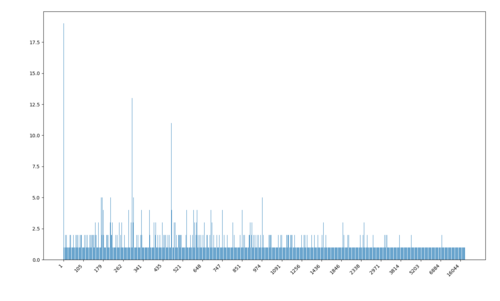
\includegraphics[width=13cm]{histo}
\end{center}
\end{figure}

Plut\^ot que garder toutes les valeurs apparues pour $l(x)$ nous les regroupons
dans des intervalles $[i_k,s_k]$ telles que pour tout intervalle d\'ecrit par
son indice $k$,
$\text{Card}\left(\left\{\ x\ |\ l(x)\in [i_k,s_k\right\}\right)=5$ par exemple
(voir F\textsc{igure} \ref{fig:histo5corpus}).

\begin{figure}[h!]
\begin{center}
    \caption{Estimation regroup\'ee des distributions pour la description par longueur}
    \label{fig:histo5corpus}
    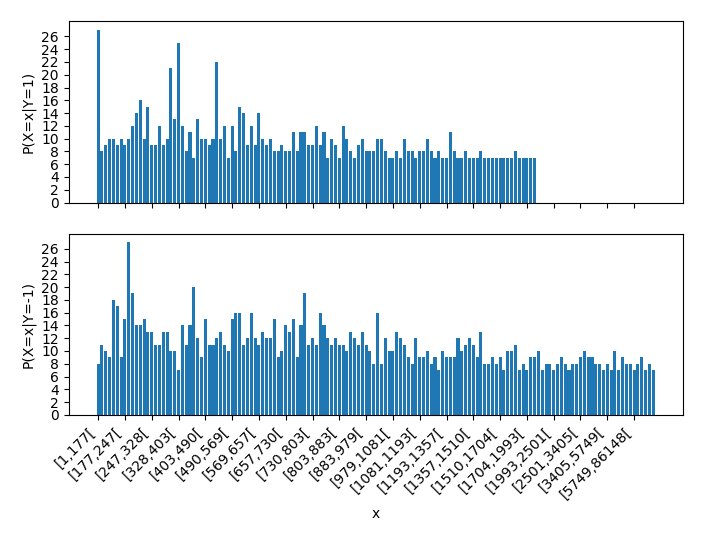
\includegraphics[width=13cm]{histo5}
\end{center}
\end{figure}

\pagebreak
Nous avons donc valid\'e la phase d'apprentissage sur le corpus $E$ et obtenu
le mod\`ele $\Theta(E)$ d\'efini par deux fonctions:
$e\colon\mathbb{N}\rightarrow [0,1]$ l'estimation de probabilit\'e
pour les email $x$ d\'ecrits pour $l(x)$ sachant que $x$ est un spam
et $\overline{e}\colon\mathbb{N}\mapsto [0,1]$ l'estimateur sachant qu'il ne s'agit
pas d'un spam; et par $p=\text{Card}\left(\left\{(x,y)\in E\ |\ y=1\right\}\right)/%
\text{Card}(E)$ (et $\overline{p}=1-p$).

Plus pr\'ecis\'ement, les fonctions $e$ et $\overline{e}$ sont d\'efinies
sur une partition finie de $\mathbb{N}$ comme indiqu\'e
pour construire les intervalles $[i_k,s_k]$ dont il est question plus haut.
La pr\'ediction s'\'evalue avec le signe de l'expression
\begin{equation}
    e(\hat{x}) \cdot p - \overline{e}(\hat{x}) \cdot (1-p)
\end{equation}
avec les notations d\'ecrites. Donc en pratique on retournera l'estimation
sur l'intervalle appris dans lequel $\hat{x}=l(x)$ se trouve. C'est justement ce
qui a \'et\'e impl\'ement\'e pour ce cas de figure o\'u le descripteur $D$ est
une fonction dont les images sont finies et sont des parties $\mathbb{N}$.

Pour finir d'illustrer avec l'\'etude de ce premier classifieur, nous souhaitons
valider ou infirmer ses valeurs de pr\'edictions. Pour ce faire nous divisons
l'ensemble $E$ d'apprentissage en deux sous-ensembles $A$ et $T$.
L'ensemble $A$ pour la phase d'apprentissage et l'ensemble $T$ pour
estimer l'erreur des pr\'edictions. Pour cette d\'emonstration,
nous choisissons arbitrairement $80\%$ des emails \'etiquet\'es dans $E$
pour constituer $A$ et les emails restants constituent $T$. Ce choix arbitraire
est alors r\'ealis\'e 40 fois et \`a chaque d\'ecoupage nous notons le nombre
de pr\'edictions incorrectes. La moyenne de la probabilit\'e d'erreur et
le score du meilleur classifieur sont pr\'esent\'es dans la T\textsc{able}
\ref{tbl:erreur_exo2}.

\begin{table}[h]
\begin{center}
    \caption{Estimation de l'erreur}
    \label{tbl:erreur_exo2}
    \vskip 4mm
    \begin{tabular}{ccc}
        &min$_f(P(f(x)\neq y))$&en moyenne\\
        sur $T$&0.5454124189063948&0.5641682113067655\\
        sur $A$&0.48148148148148145&0.515787037037037
    \end{tabular}
\end{center}
\end{table}

Autant dire que les mod\`eles appris avec une telle application de description
ne sont pas fiables. Cependant, ce mod\`ele nous a permis de d\'etailler chaque
phase dans la r\'esolution du probl\`eme de classification pos\'e. Nous allons
nous porter plus longtemps \`a pr\'esent sur le choix de la description $D$
pour compl\'eter le manque d'informations qui nous emp\^eche
d'inf\'erer correctement la classe \`a laquelle appartient un email.


\section{Description vectorielle d'emails, repr\'esentations, cas limites}

L'objet d'\'etude, ici, est de r\'efl\'echir et d'\'evaluer la performance
de mod\`eles appris sur des descriptions enrichies.

Avec la description que nous avions choisi pour l'exemple de la
premi\`ere partie nous avons omis jusque l\`a le corps de l'email.
Il pourrait s'agir sur papier de d\'ecomposer le corps en mots et
de repr\'esenter un email $x=\left(x_{i_1},x_{i_2},\ldots,x_{i_{l(x)}}\right)$
avec $\mathcal{D}=\left\{x_1,x_2,\ldots,x_d\right\}$ le dictionnaire des $d$
mots possiblement trouvables dans un email.
Nous pouvons imaginer plusieurs descriptions pour cette
repr\'esentation de $x$ :
\begin{align*}
    \label{eq:description_vect}
    D_0(x) = &\left(\mathbb{I}_x[x_{i}]\right)_{i\in\{1,\cdots,d\}}\\
    D_1(x) = &\left(\mathbb{I}_x[x_{i},x_{j}]\right)_{i\neq j\in\{1,\cdots,d\}}\\
             &\cdots\\
    D_n(x) = &\left(\mathbb{I}_x[x_{i_1},x_{i_2},\ldots.x_{i_n}]\right)%
    _{i_1\neq i_2\neq \cdots \neq i_n\in\{1,\cdots,d\}}
\end{align*}
o\`u $\mathbb{I}_x[x_{i_1},x_{i_2},x_{i_n}]$ vaut $1$ si $x$ contient
la sous-s\'equence de mots $(x_{i_1},x_{i_2},\ldots,x_{i_n})$ et $0$ sinon.

Par intuition, $D_0$ est une description moins riche que $D_1$, $\ldots$,
$D_n$, avec pour hypoth\`ese tr\`es raisonnable que $n<<d$.
Mais il en est pas des moindres d'envisager de les impl\'ementer.
En effet la complexit\'e pour repr\'esenter l'estimation $P(X=D_0(x)|Y)$
en m\'emoire est en $O(2^d)$ puisque nous repr\'esenterons les valeurs de
probabilit\'es pour les \'eventuelles $2^d$ descriptions dans
$\left\{0,1\right\}^d$. Sur les corpus \cword{spam}, \cword{nospam}
fournis, on d\'enombre $53808$ mots. C'est \`a dire qu'il serait n\'ecessaire
d'avoir une structure de donn\'ees donnant l'acc\`es \`a $2^{53808}$
, et autrement dit environs $10^{1800\cdot9}$ flottants.

Face \`a ce probl\`eme nous pouvons ou bien \'etudier
l'ind\'ependance des variables al\'eatoires $X_i=\mathbb{I}_x[x_i]$
et en conservant la description $D_0$ stocker l'estimation $P(X=D_0(x)|Y)$
avec $O(d)$ flottants $P(X_i=\mathbb{I}_x[x_i]|Y)$, ou bien r\'eduire $d$
\`a partir d'une heuristique parce que la borne $2^d$ reste tr\`es pessimiste.

Faute de quoi, on peut s'apercevoir qu'il n'est pas n\'ecessaire de
consid\'erer $\mathcal{D}$ dans sa totalit\'ee aussi bien qu'il n'est pas
n\'ecessaire de sauvegarder toutes les combinaisons possibles d'apparitions
parce que nombre d'entre elles sont nulles i.e. impossibles de la perspective
de l'ensemble d'apprentissage.

\begin{figure}[h]
\begin{center}
    \caption{Fr\'equences des mots dans le corpus}
    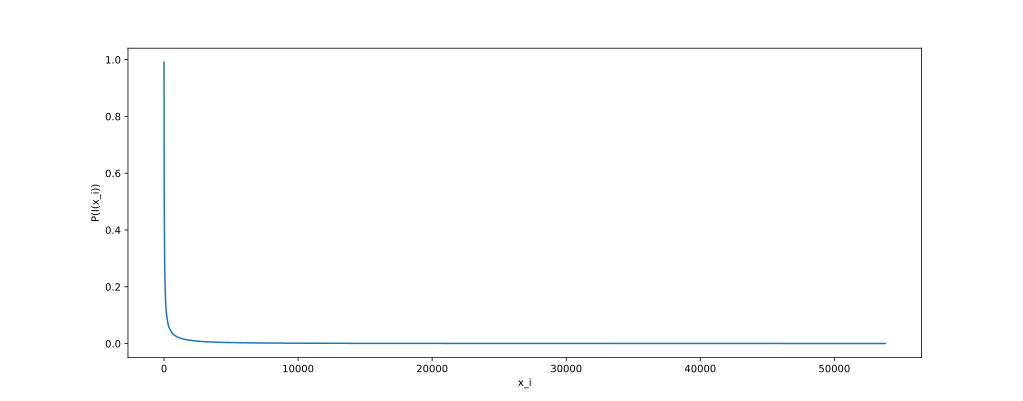
\includegraphics[width=13cm]{repr0}
\end{center}
\label{fig:repr0}
\end{figure}

La F\textsc{igure} \ref{fig:repr0} propose une premi\`ere heuristique qui est de
ne pas consid\'erer les mot trop peu apparus avec chacune des indicatrices au
del\`a des 5000 premiers mots de $\mathcal{D}$ et de ne pas consid\'erer les
mots trop fr\`equents  apparus dans l'ensemble d'apprentissage non plus. D\`es
\`a pr\'esent nous concentrerons nos efforts sur  $D_{\sigma,\overline\sigma}$
la description pour un email sur le sous-ensemble significatif de $\mathcal{D}$,
$\sigma$, pour lequel nous pourrions estimer non exhaustivement et
raisonnablement les combinaisons apparues. Donc il s'agit de la restriction de
$D_0$ sur $\sigma$; et d'autre part prolong\'ee sur le sous-ensemble non
significatif $\overline\sigma$ sur lequel on pr\'esentera plus loin des
alternatives sous des hypoth\`ese faibles d'ind\'ependance. On nomme se couple
$(\sigma, \overline\sigma)$ la repr\'esentation du corpus.

Quand il s'agira de proposer une description dans ce contexte, nous distinguerons
\begin{itemize}
    \item l'estimation bas\'ee sur le descripteur $D_\sigma$ avec, par exemple
        $\sigma$ les 500 mots les plus fr\'equents
    \item l'estimation bas\'ee sur les 500 premiers descripteurs $D_{i,\sigma}$
        pour chacun de ces 500 mots de $\sigma$.
\end{itemize}


\vskip 4mm
D'ailleurs nous nous proposons de visualiser empiriquement si le produit des
distributions ind\'ependantes des $P(X_i=D_{i,\sigma}(x)|Y)$  est proche de la distribution
de $P(X=D_{\sigma}(x)|Y)$ pour le corpus donn\'e. Nous r\'ealisons autant d'estimations
qu'il y a de blocs successifs de 500 mots dans $\mathcal{D}$ tronqu\'e au mot 10000.
%
Il s'agit de 20 blocs, la complexit\'e empirique du nombre d'estimations
pour chaque bloc se lit T\textsc{able} \ref{table:combinaisons_decalages}).
%
Nous prenons les mots dans l'ordre des plus fr\'equents aux moins fr\'equents.

\begin{table}[h]
\begin{center}
    \caption{\'Evaluation empirique de la complexit\'e de repr\'esentation}
    \label{table:combinaisons_decalages}
    \vskip 4mm
    \begin{lstlisting}
        [0:10] 855, 782, 735, 674, 618, 563, 495, 481, 451, 408
        [10:20] 380, 380, 337, 333, 335, 306, 272, 289, 259, 261
    \end{lstlisting}
    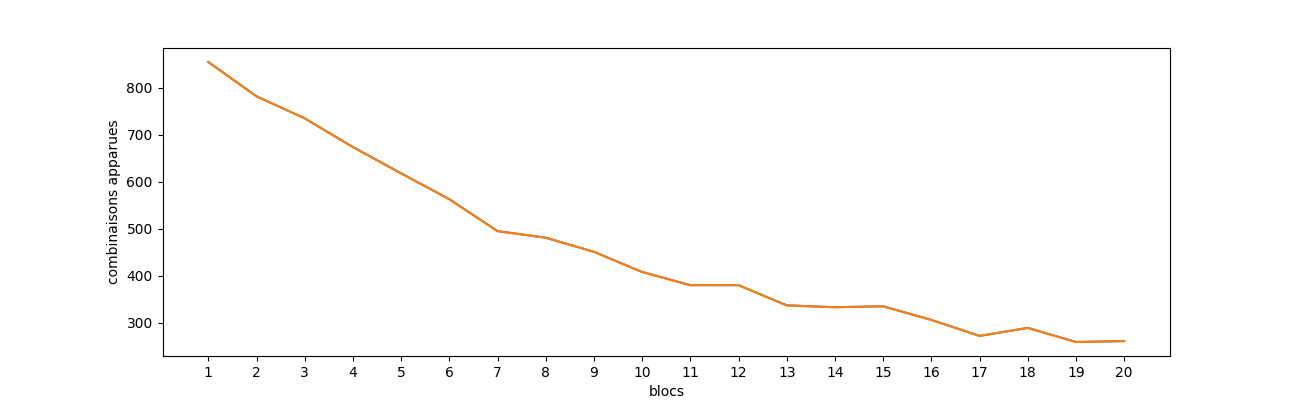
\includegraphics[width=12cm]{cn_decalages}
\end{center}
\end{table}

Le premier constat empirique est que la complexit\'e de $D_\sigma$ \`a \'et\'e
surestim\'ee par $2^d$ dans ce cas pratique avec Card$(\sigma)=500$. De plus,
on visualise ici que l'information inf\'er\'ee sur le corpus est moindre sur
les tranches de mots moins fr\'equents.
%
Pour la repr\'esentation sur les 10000 premiers mots de $\mathcal{D}$,
nous pourrions plut\^ot que consid\'erer les estimations avec $D_{\sigma}$
consid\'erer les 20 estimations sur ces blocs avec $D_{\sigma_i}$ o\`u
$\sigma_i$ correspond \`a un bloc et supposer ces distributions
ind\'ependantes.
Cette derni\`ere hypoth\`ese est moins forte que si on suppose
l'ind\'ependance sur des blocs de taille 1.

Le calcul des distributions pour chaque repr\'esentation ${\sigma_i}$,
$1\leq i\leq 20$, pour les 20 blocs de 500 mots et le calcul des distributions
pour chaque repr\'esentation en supposant l'ind\'ependance
(donc 20 vecteurs de taille 500) sont r\'ealis\'es s\'epar\'ements en exploitant
les features de la librairie \cword{multiprocessing} de \cword{python3}
et en utilisant le module \cword{numpy}.
Nous sauvegardons ces donn\'ees sur le corpus dans des fichiers qui finalement,
rappelons-le, d\'ecrivent l'ensemble des param\`etres pour construire le
mod\`ele $\Theta(E)$.

En termes d'impl\'ementation, l'estimation d'une repr\'esentation $\sigma_i$
\emph{suppos\'ee ind\'ependante} est une liste de taille Card$(\sigma_i)$
des probabilit\'es $P(X=D_{j,\sigma_i}(x)|Y=y)$, $1\leq j\leq \text{Card}(\sigma_i)$,
pour chaque label $y\in\left\{-1,+1\right\}$ et estim\'ee sur les $x$ de $E$.
D'autre part, l'estimation d'une repr\'esentation $\sigma_i$ est un dictionnaire
dont les cl\'es sont les cha\^ines de caract\`eres de tailles
Card$(\sigma_i)$ compos\'ees de \cword{0} et \cword{1}
qui pointent vers les probabilit\'es $P(X=D_{\sigma_i}(x)|Y=y)$ --
ces choix d'impl\'ementation se justifient du fait que
$D_{\sigma_i}(x)\in\left\{0,1\right\}^{\text{Card}(\sigma_i)}$ et
que $D_{j,\sigma_i}(x)\in\left\{0,1\right\}$.

\begin{figure}[h]
\begin{center}
    \caption{%
    $\Delta_{+1}(x)=\left|
    \prod _j P(X=D_{j,\sigma_i}|Y=+1)-P(X=D_{\sigma_i}|Y=+1)\right|(x)$}
    \label{fig:blocs_indes_spam}
    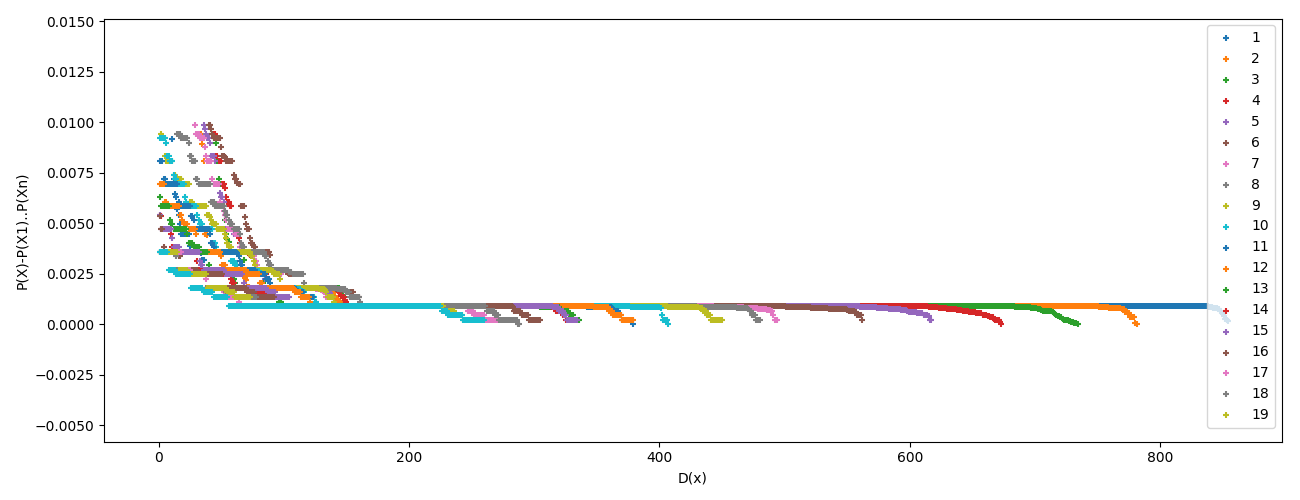
\includegraphics[width=13cm]{blocs_indes_spam}
\end{center}
\end{figure}
\begin{figure}[h]
\begin{center}
    \caption{%
    $\Delta_{-1}(x)=\left|
    \prod _j P(X=D_{j,\sigma_i}|Y=-1)-P(X=D_{\sigma_i}|Y=-1)\right|(x)$}
    \label{fig:blocs_indes_nospam}
    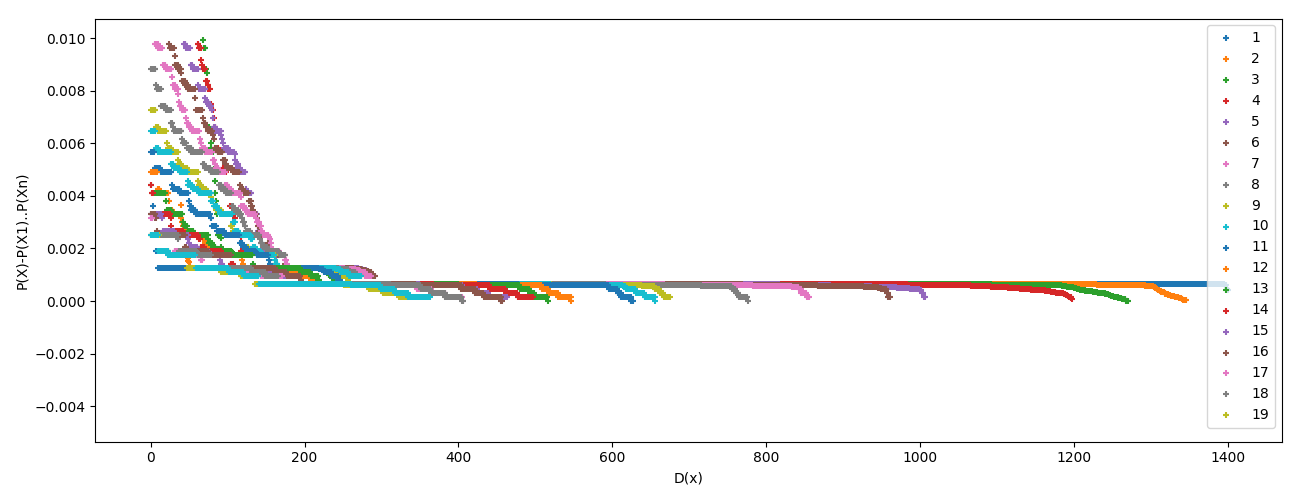
\includegraphics[width=13cm]{blocs_indes_nospam}
\end{center}
\end{figure}

Nous avons calcul\'e pour chaque bloc la diff\'erence de probabilit\'e
sous chacune des hypoth\`eses. Les diff\'erences sont trac\'ees sur la
F\textsc{igure} \ref{fig:blocs_indes_spam} et la F\textsc{igure}
\ref{fig:blocs_indes_nospam} si elle est inf\'erieure \`a $10^{-2}$
pour les estimations des repr\'esentations $\sigma_i$, $1\leq i\leq 19$.
On en d\'eduit que l'hypoth\`ese d'ind\'ependance des $X_j=D_{j,\sigma_i}$
est trop forte pour inf\'erer un bon mod\`ele et surtout sur les blocs des
mots les plus fr\'equents. On pourra se faire une id\'ee plus fine
des ind\'ependances en fonction de $\sigma_i$ le bloc de mots
\'evalu\'e avec la F\textsc{igure} \ref{fig:seuils_indes_spam} et
la F\textsc{igure} \ref{fig:seuils_indes_nospam} qui pour chaque classe
et chaque bloc indiquent le nombre de cl\'es pour lesquelles ont doit
r\'efuter l'hypoth\`ese pour un seuil $\Delta_y(x)<10^{-2}$.

\begin{figure}[h]
\begin{center}
    \caption{Seuils d'ind\'ependances pour le corpus spam}
    \label{fig:seuils_indes_spam}
    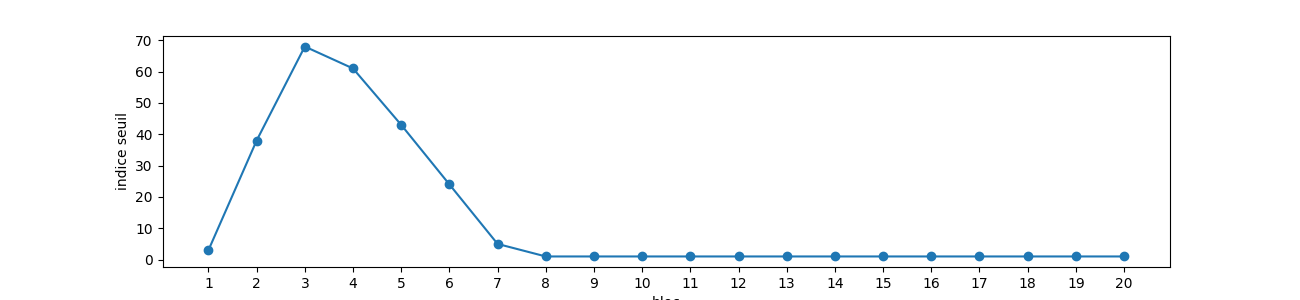
\includegraphics[width=15cm]{seuils_indes_nospam}
\end{center}
\end{figure}

\begin{figure}[h]
\begin{center}
    \caption{Seuils d'ind\'ependances pour le corpus nospam}
    \label{fig:seuils_indes_nospam}
    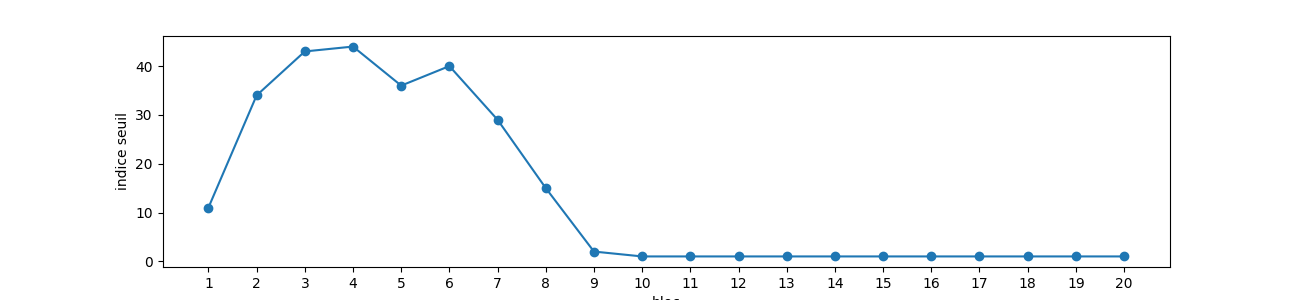
\includegraphics[width=15cm]{seuils_indes_spam}
\end{center}
\end{figure}

Cette analyse nous conduit \`a ne surtout pas faire l'hypoth\`ese
d'ind\'ependance sur les premiers descripteurs correspondants aux mots
les plus fr\'equents. Aussi plus les probabilit\'es sont faibles, plus il
est possible que les valeurs transf\`erent une erreur d'estimation suite \`a
plusieurs op\'erations num\'eriques. \`A ce sujet, nous avons pris quelques
pr\'ecautions comme faire priorit\'e aux additions et soustractions face aux
multiplications et aux divisions et donc privil\'egi\'e le passage au
logarithme comme avec \eqref{eq:logprod} ce qui permet de r\'eduire les erreurs.

\begin{equation}
    \text{log}\left(\prod _i p_i\right) = \sum _i \text{log}(p_i)
    \label{eq:logprod}
\end{equation}

\`A pr\'esent, nous avons pos\'e les notations qui nous permettent
de d\'ecrire les diff\'erentes repr\'esentations envisageables pour
construire un mod\`ele d'inf\'erence sur un ensemble d'apprentisage;
et nous avons visit\'e sur un corpus d'exemples d'apprentissages les
\'ecueils qui pourraient nuire \`a la qualit\'e du mod\`ele ou le rendre
discutable pour sa complexit\'e. Cependant, et nous l'avons observ\'e
plusieurs fois, restreindre la description \`a un sous-ensemble $\sigma$
de mots n'est pas satisfaisant parceque l'on perds une quantit\'e non
n\'egligeable d'information.

\section{Enrichissement au moindre co\^ut : notre mod\`ele}

Apr\`es avoir parcouru le registre des descripteurs, dans cette partie
nous pr\'esentons le classifieur contruit sur une description \'etendue
avec une repr\'esentation $\left(\sigma(E),\overline\sigma(E)\right)$ \'evalu\'ee
selon $E$ au d\'ebut de l'apprentissage.

Nous pr\'esenterons d'abords les crit\`eres et la proc\`edure
pour constuire cette repr\'esentation. C'est le couple de deux ensembles :
un ensemble de mots et un ensemble des parties des mots laiss\'es de c\^ot\'e;
qui nous permettra par la suite de constuire
un mod\`ele $\Theta(E)$ avec une estimation d'erreur faible.

Nous devrons \`a mi-temps pr\'esenter un dernier descripteur
$D_{\overline\sigma}$.

\subsection{Constuire une repr\'esentation $\sigma, \overline\sigma$ satisfaisante}

Reprenons \`a la F\textsc{igure} \ref{fig:repr0} : c'est l'allure de la courbe
des fr\'equences d'apparition des mots dans le corpus qui nous fait induire
que les mots trop fr\'equemment pr\'esents augmentent non significativement
la complexit\'e pour repr\'esenter le mod\`ele d'autant que ces mots sont tr\`es
succeptibles d'augmenter le nombre de combinaisons $D_\sigma(x)$ quand on visite
$E$ pour apprendre le mod\`ele. D'autre part, nous avons vu qu'au del\`a
des 10000 premiers mots les plus fr\'equents, les mots sont pr\'esent
tr\`es sp\'ecifiquement pour peu d'exemples du corpus.

La proc\'edure pour constituer la repr\'esentation $(\sigma,\overline\sigma)$
qui nous int\'eresse ce d\'ecompose en trois \'etapes

\begin{enumerate}
  \item vider $\mathcal{D}$ des mots facteurs de bruit parce qu'ils
  apparaissent trop fr\'equement,\\
  on notera $\mathcal{D}^0$ le nouveau dictionnaire
  \item d\'eterminer l'ensemble $\sigma$\\ en recoupant avec un nombre
  raisonable des mots les plus fr\'equents de $\mathcal{D}^0$,\\
  on notera $\mathcal{D}^{\sigma}$ le dictionnaire obtenu et\\ il reste
  $\mathcal{D}^1$ le dictionnaire des mots les moins significativement
  importants
  \item choisir une partition de $\mathcal{D}^1$ satisfaisante dont on
  d\'eduit  d\'eduire $\overline\sigma$
\end{enumerate}

Supposons que nous avons d\'ej\`a d\'eterminer $\sigma$ et que nous arrivons
\`a la derni\`ere \'etape avec $\mathcal{D}^1=\left\{x_1,\ldots,x_n\right\}$
tel que $f(x_1)\geq\ldots\geq f(x_n)$. Alors $n$ est certainement encore tr\`es
grand. Nous aurions int\^eret \`a r\'esumer l'information sur des parties
succesives de $\mathcal{D}^1$. Pour d\'eterminer les tranches, nous posons la
suite des $n-1$ \'el'ements $d_i\colon i\mapsto f(x_{i+1})-f(x_i)$.
Les valeurs qui nous interessent sont les valeurs de $i$ telles que $d_i<0$.
Alors que $n$ est grand, $f(x_1)$ est petit et de plus en plus commun\'ement,
les $x_i$ sont de m\^eme fr\'equence et donc $d_i=0$ pour ces valeurs.
Si on note $(i_1, i_2, \ldots i_k)$ les valeurs de $i$ pour lesquelles $d_i<0$
on obtient les indices qui d\'elimitent les tranches de mots
donnant en moyenne la m\^eme quantit\'e d'information.

Avec les notations utilis\'ees, la repr\'esentation
\begin{equation}
    \overline\sigma=\left\{
        \left\{
            x_{i_1},\ldots,x_{i_2}
        \right\},
        \left\{
            x_{i_2+1},\ldots,x_{i_3}
        \right\},
        \ldots,
        \left\{
            x_{i_{k-1}+1},\ldots,x_{i_k}
        \right\}
    \right\}
\end{equation}
sugg\`ere une description moins lourde qui apporte une information
suppl\`ementaire pour le mod\`ele. Nous choisissons
\begin{equation}
    D_{j,\overline\sigma}\colon
    x\mapsto
    \sum_{i=i_j}^{i_{j+1}} \mathbb{I}_{x}[x_{i}]
\end{equation}
les $k$ descripteurs \`a valeurs dans $\mathbb{N}$ comptant le nombre de
mots apparues dans un email $x$ dans la tranche $[i_j,i_{j+1}[$ de
$\overline\sigma$. Avec le m\^eme corpus que dans les parties pr\'ec\'edentes
nous convenons par tatonnement que si la d\'eriv\'ee discr\`ete de
la fr\'equence est strictement n\'egative plus de 500 fois sur un intervalle
alors on peut le consid\'erer comme un partie de $\overline\sigma$.

On utilise un criti\`ere similaire pour d\'eterminer l'ensemble des mots
significativement pr\'esents dans $\mathcal{D}^0$ : on consid\`ere les
mots dont les fr\'equences ordonn\'ees du plus au moins fr\'equents est
au moins strictement d\'ecroissante sur des intervalle de 10 mots. Ainsi
on se limitera \`a une repr\'esentation $\sigma$ de taille 642 mots ce qui
est satisfaisant d'apr\`es la partie 2.

Finalement nous avons retranch\'e arbitrairement \`a la premi\`ere \'etape les
mots trop fr\'equents \`a l'\'etape 1 en selectionnant les mots dont la
fr\'equence est inf\'erieure \`a $\frac{1}{2}\cdot$Card$(\{Y=1\})/$Card$(E)$.

\subsection{Notre mod\`ele : 0.05 pr\'edictions \'eronn\'ees en moyenne}

Exactement \`a l'image de la premi\`ere partie l'ensemble d'apprentissage
est divis\'e al\'eatoirement et arbitrairement en deux sous-ensemble de $E$ :
les exemples de test $T$ (30\%) et les exemples d'apprentissage $A$ (70\%).

Apr\`es avoir \'evalu\'e la repr\'esentation
$\left(\sigma,\overline\sigma\right)$ sur $A$, l'apprentissage se d\'ecompose
en deux parties ind\'ependantes :
le calcul des estimations pour la description $\sigma$ et
le calcul des estimations pour les descriptions de $\overline\sigma$.

En moyenne, l'estimation des probabilit\'es $P(D_{\sigma}|Y)$ sur les
corpus \cword{spam} et \cword{nospam} (2698 emails) s'op\`ere sur une
repr\'esentation de 500 \`a 680 mots relativement rapidement. D'autre
part, pour chaque partie $\overline\sigma_i$ de $\overline\sigma$ nous
somme ramen\'es au cas de la premi\`ere partie parce que les descripteurs
$D_{i,\overline\sigma}$ correspondants sont des applications \`a valeurs dans
$\mathbb{N}$. Alors, pour s'assurer de pouvoir estimer la probabilit\'e
correspondante et repr\'esenter en m\'emoire cette distribution, nous
devons calculer un regroupement des valeur prisent par les descriptions.
Cela dit, le mod\`ele apprend en un temps raisonable malgr\`es que cette
second partie est relativement plus co\^uteuse en temps de calul.

Les r\'esultats pour les calculs de ces deux repr\'esentations sont suppos\'es
ind\'ependants puisque lorsqu'il s'agit de calculer $P(X=x|Y=y)$ on \'evalue
\begin{equation}
  P(X=D_\sigma(x)|Y=y)\prod_{i} P(X=D_{i,\overline\sigma}(x)|Y=y).
\end{equation}

En exploitant les features des outils \cword{multiprocessing} et
\cword{multiprocessing.dummy} de \cword{python3}, le mod\`ele $\Theta(A)$
est appris et test\'e sur $T$ globalement en 4 minutes (T\textsc{able}
\ref{tbl:time_modeleplus}).

\begin{table}[h]
\begin{center}
  \caption{Temps pour apprendre et tester le mod\`ele}
  \vskip 4mm
  \begin{tabular}{rl}
    real    &0m40.460s\\
    user    &3m26.552s\\
    sys     &0m6.872s
  \end{tabular}
  \label{tbl:time_modeleplus}
\end{center}
\end{table}

Nous avons entra\^in\'e 11 mod\`eles avec, \`a chaque fois, un d\'ecoupage
diff\'erent de $E$. En moyenne un mod\`ele pr\'edit correctement 94.29\%
des emails. Le meilleur mod\`ele entra\^in\'e sur cette repr\'esentation
du corpus se trompe dans 5.19\% des cas.

\paragraph{Conclusion --}
Nous avons du trouver un compromis pour repr\'esenter un email au risque de ne
pas pouvoir calculer les distributions de probabilit\'es n\'ecessaires pour
pr\'edire au mieux si un nouvel email est un spam ou ne l'est pas. Ce compromis
est r\'ealis\'e parce que nous avons fait les choix de cette repr\'esentation.
C'est sur ces choix que nous devrions r\'efl\'echir si nous souhaiterions
am\'eliorer les mod\`eles ou r\'ealiser qu'ils sont suffisament satisfaisant
\`a l'\'egard de cette approche.


%\end{multicols}
\end{document}
